\section{Versuchsaufbau und Durchführung} % (fold)
\label{sec:versuchsaufbau_und_durchf_hrung}

	\subsection{Aufbau des Michelson-Interferometers} % (fold)
	\label{sub:aufbau_des_michelson_interferometers}

	\begin{figure}[htb]
		\centering
		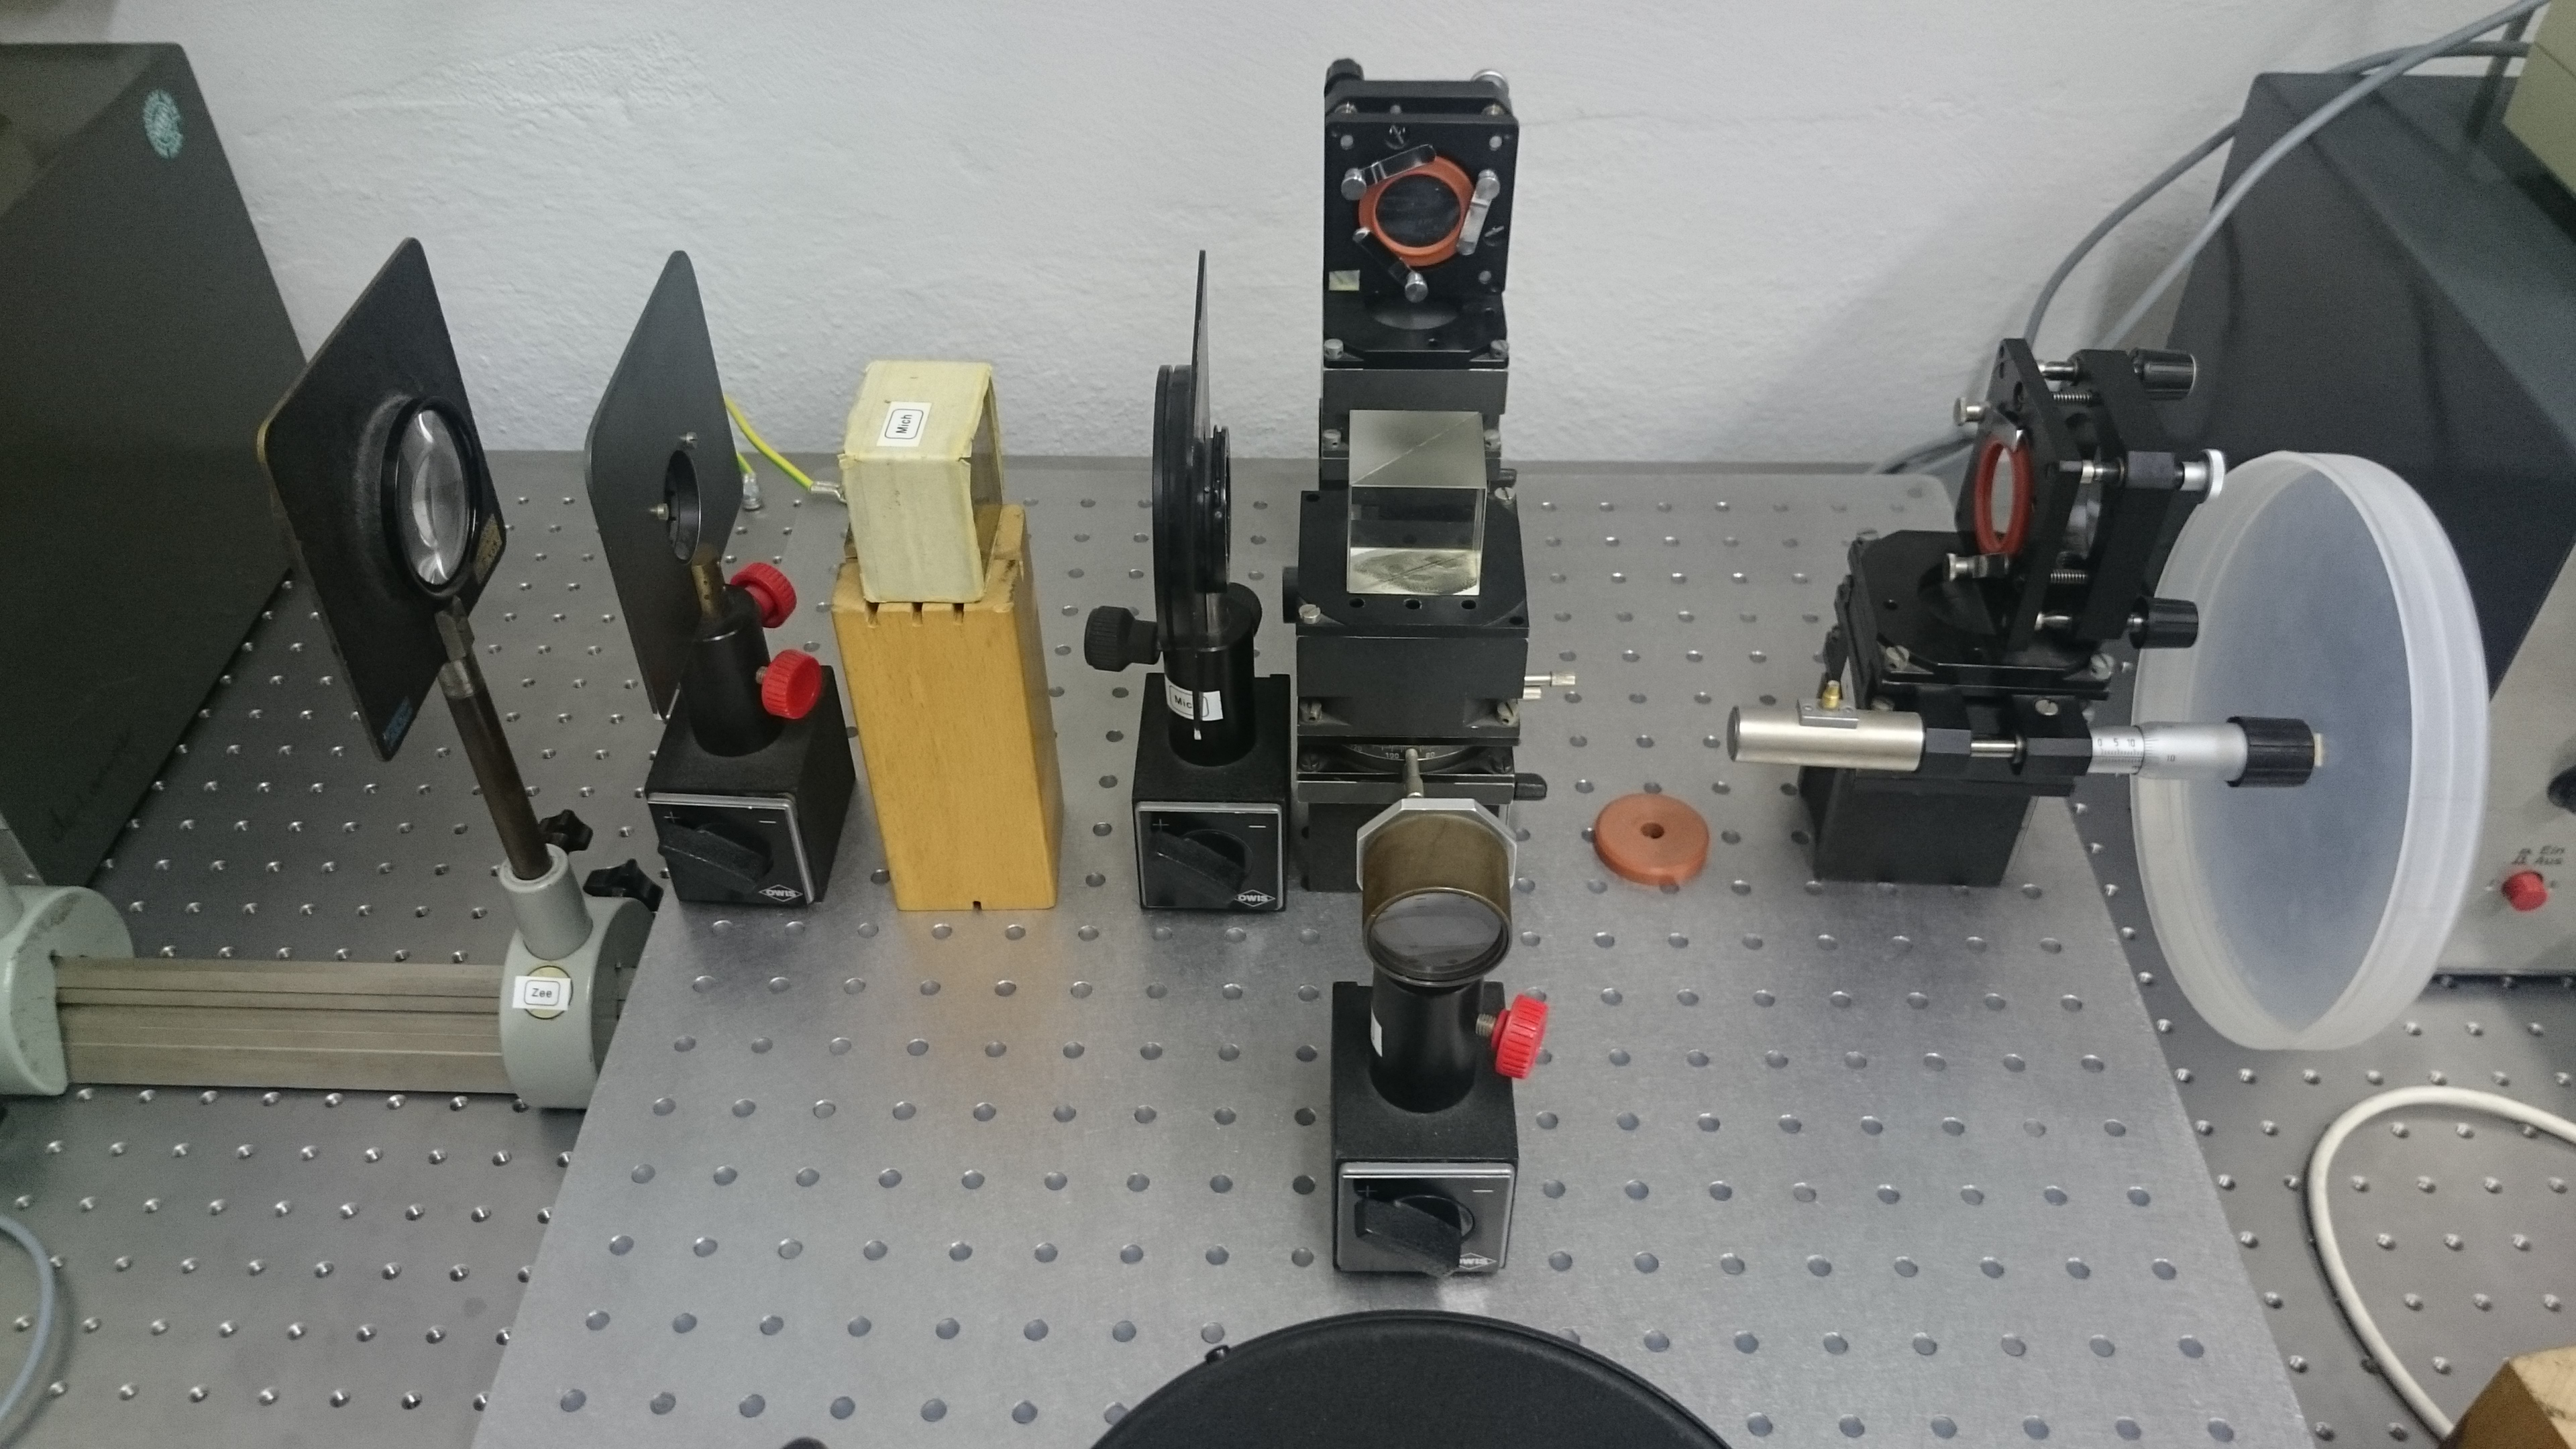
\includegraphics[scale = 0.08]{images/DSC_1011.JPG}
		\caption{Montagetisch mit Versuchsaufbau des MIF}
		\label{fig:aufbau-mif-1}
	\end{figure}

	In Abbildung \ref{fig:aufbau-mif-1} ist der Aufbau des MIF zu sehen, wie er unter Abschnitt \ref{sub:prinzip_des_michelson_interferometers} beschrieben wurde.
	Als Lichtquelle können eine Hg-Dampflampe mit verschiedenene Filtern sowie eine herkömmliche Glühlampe verwendet werden.
	Spiegel 2 ist über eine Mikrometerschraube in x-Richtung zu verstellen, drei weitere Feingewindeschrauben sind für die Winkeleinstellung vorgesehen.
	Durch Verwendung des Strahlteilerwürfels entfällt die sonst notwendige Kompensationsplatte.
	Neben der direkten Möglichkeit zur Beobachtung durch Blicken in den Strahlteiler, kann der Strahl auch noch mittels einer weiteren Linse und eines Ablenkspiegels auf Papier abgebildet und abfotografiert werden.
	
	% subsection aufbau_des_michelson_interferometers (end)


	\subsection{Aufbau des Fourier-Spektrometers} % (fold)
	\label{sub:aufabu_des_fourier_spektrometers}
	

	\begin{figure}[htb]
		\centering
		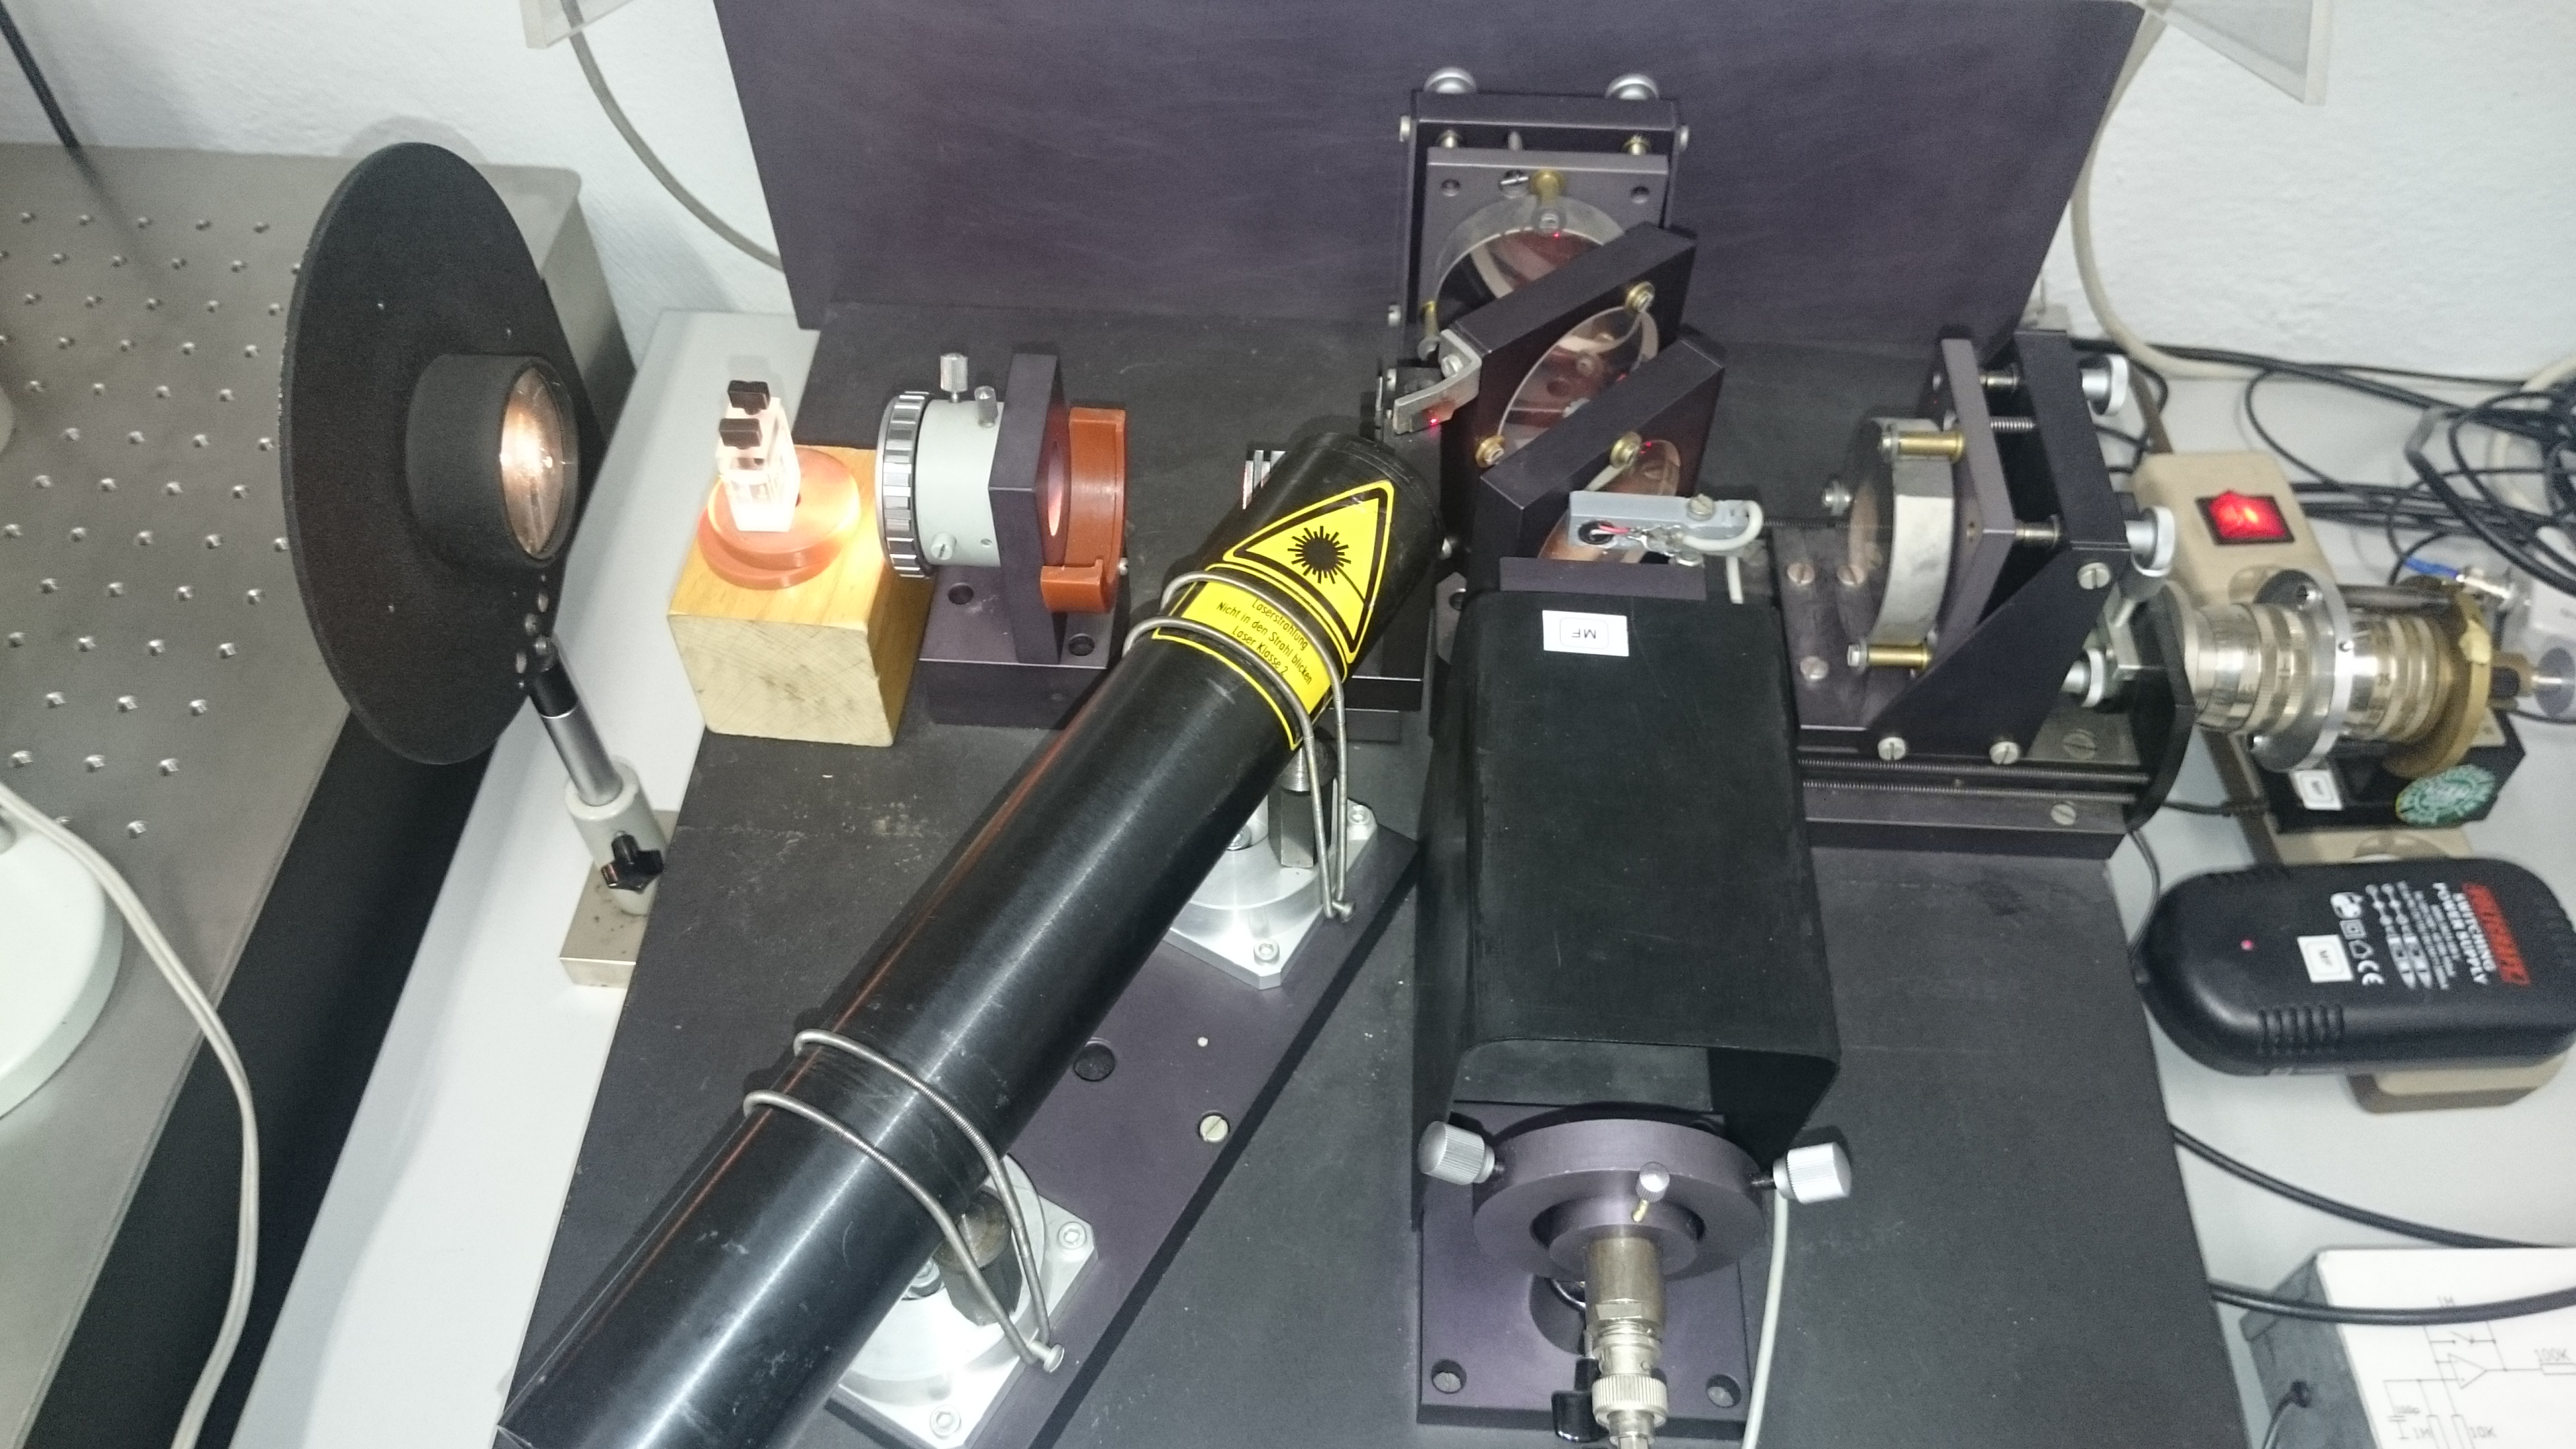
\includegraphics[scale = 0.08]{images/DSC_1010.JPG}
		\caption{Komponenten des Fourier-Spektrometers mit geöffneter Abdeckklappe}
		\label{fig:aufbau-mif-2}
	\end{figure}

	Abbildung \ref{fig:aufbau-mif-2} zeigt alle Komponeneten des Fourierspektrometers wie es im Versuch verwendet wurde.
	Links befindet sich die Lichtquelle.
	Als solche werden im Versuch Hg-Lampe, Na-Lampe, grüne LED, rote Laser-LED, Gas-Laser und Glühlampe verwendet.
	Zwischen Lampe und Kollimator können Filter oder Proben zur Absorbtion platziert werden.
	In der Mitte teilt ein halbdurchlässiger Spiegel den Strahl, kurz darüber ist die Kompensationsplatte zu finden.
	Spiegel 2 kann mittels einer Mikrometerschraube und den dahinter befindlichen Motor über den Computer gesteuert werden.
	Unter dem Strahlteiler befindet sich eine Linse, die den Strahl auf den Detektor bündelt.
	Auf der Linse befindet sich der Detektor für das Laser-Referenzsignal.
	An diesem wird die Messung anschließend angepasst und kalibriert.
	Akkumulierung der Datenpunkte, Aufzeichnen des Interferogramms und Erstellen der zugehörigen FFT (Fast Fourier Transformation) werden von einem LabView-Programm erledigt.
	Es dient ebenfalls zum Ansteuern des Motors von Spiegel 2.

	% subsection aufabu_des_fourier_spektrometers (end)


% section versuchsaufbau_und_durchf_hrung (end)